%\documentclass{beamer}
%\usetheme{Pittsburgh}
\documentclass{scrartcl}

\usepackage[utf8]{inputenc}
\usepackage{default}
\usepackage[procnames]{listings}
\usepackage{graphicx}
\usepackage{adjustbox}
%\usepackage[toc,page]{appendix}
\usepackage{caption}
\usepackage{hyperref}
\usepackage{color}
%\usepackage{csvsimple}
\usepackage{float}
%\usepackage[T1]{fontenc}



%Bibliogrpahy?
%\usepackage{bibentry}
%\nobibliography*
%\bibentry{ }


%Python
\definecolor{keywords}{RGB}{255,0,90}
\definecolor{comments}{RGB}{0,0,113}
\definecolor{red}{RGB}{160,0,0}
\definecolor{green}{RGB}{0,150,0}
\lstset{language=Python,
    basicstyle=\ttfamily\scriptsize,
    keywordstyle=\color{keywords},
    commentstyle=\color{comments},
    stringstyle=\color{red},
    identifierstyle=\color{green},
    breaklines = true,
    columns=fullflexible,
    %Numbering and tabs
    %numbers=left,
    %numberstyle=\tiny\color{gray},
    %stepnumber=2,
    %numbersep=1em,
    tabsize=4,
    showspaces=false,
    showstringspaces=false}

\begin{document}

\title{Learning and Adaptivity}
\subtitle{Final Report}
\author{
  \href{daiem.ali@smail.inf.h-brs.de}{Ali, Daiem}: \href{https://github.com/daiemna}{github.com/daiemna}\\
  \href{christophe.quignon@smail.inf.h-brs.de}{Quignon, Christophe}:\href{https://github.com/ChrisQuignon}{github.com/ChrisQuignon}
  %Familyname, Name
}
\date{\today}


\maketitle


\begin{abstract}
\textbf{Abstract:}
Heat pumps are a sustainable way to transfer thermal energy into out away from builds to keep a comfortable temperature. But to operate a heating pump is not a trivial task, different building distribute the heat differently and weather with its chaotic nature has a major influence on the temperature flow. With an accurate prediction of the energy consumption, one can increase their efficiency and operating cost.
Thus we want to predict the behaviour or an energy pump with respect to the weather.\\
%TODO include method and conclusion
\end{abstract}

\section{Data}
\label{sec:data}
%TODO: CHECK READ
%what is the problem what is the data wheat is the purpose

The Recogizer GmbH provided me a dataset of 4 sensor reading, three weather indicators and an accumulated energy consumption. In 242 days (between July 2014 to February 2015), over 1,300,000 data points where collected.

\paragraph{Weather data:}
The regional weather is from the official recordings of the "Deutsche Wetterdienst" (German weather service) and contains:

\begin{itemize}
\item Temperature in $^\circ C$
\item Relative air humidity in percent
\item Precipitation in mm (1 litre per square meter)
\end{itemize}

\paragraph{Sensor data:}
The Measurements from the systems are:

\begin{itemize}
\item Volumetric flow rate in $m^3 / s$
\item Rate of heat flow in watts
\item Supply temperature in $^\circ C$
\item Return temperature $^\circ C$
\end{itemize}

\paragraph{Accumulated data:}
The energy in watt hours, calculated per day.

\section{Analysis}
\label{sec:analysis}

%\subsection{Correlation}
%TODO
%\begin{figure}[H]
%  %\raggedleft
%  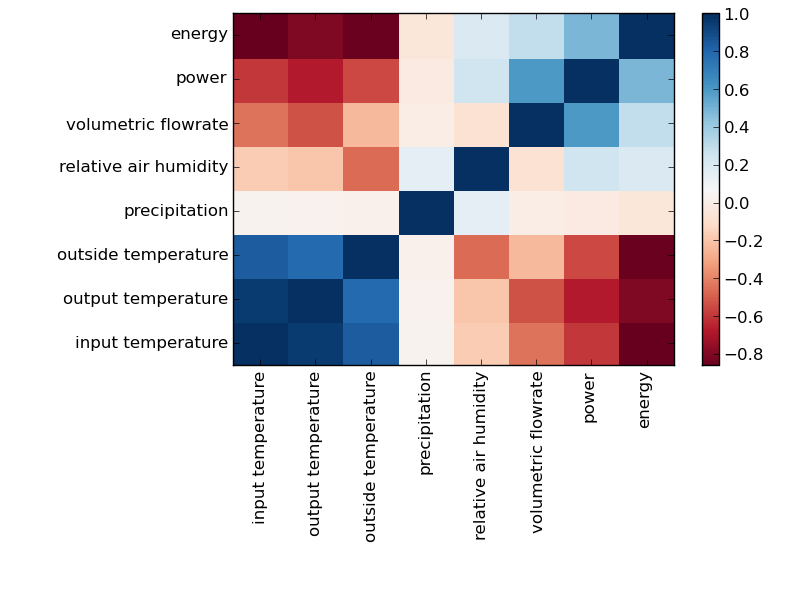
\includegraphics[width=0.6\linewidth]{img/correlation.png}
%  \caption{Correlation of the datasets.}
%  \label{fig:correlation}
%\end{figure}

\subsection{Seasonal decomposition}
%TODO
Our data has a seasonal trend which is shown in the figure \ref{fig:season_outside_temperature}. In the figure recordings of one whole week outside temperature is shown. We can see that peak is repeated every day with little offset. for this reason we introduced the day of the year(DOY) as a feature. The effect of introducing DOY in \ref{fig:RandomForestRegressor_day_error_without_some_params_DOY} 
\begin{figure}[H]
  \center
  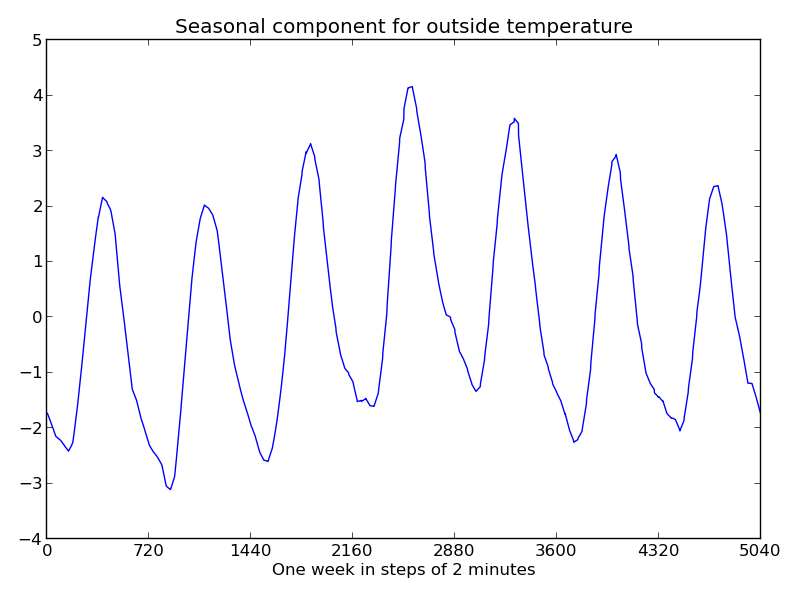
\includegraphics[width=0.6\linewidth]{img/season-outside_temperature.png}
  \caption{Seasonal (weekly) decomposition of the datasets.}
  \label{fig:season_outside_temperature}
\end{figure}



\begin{figure}[H]
  \center
  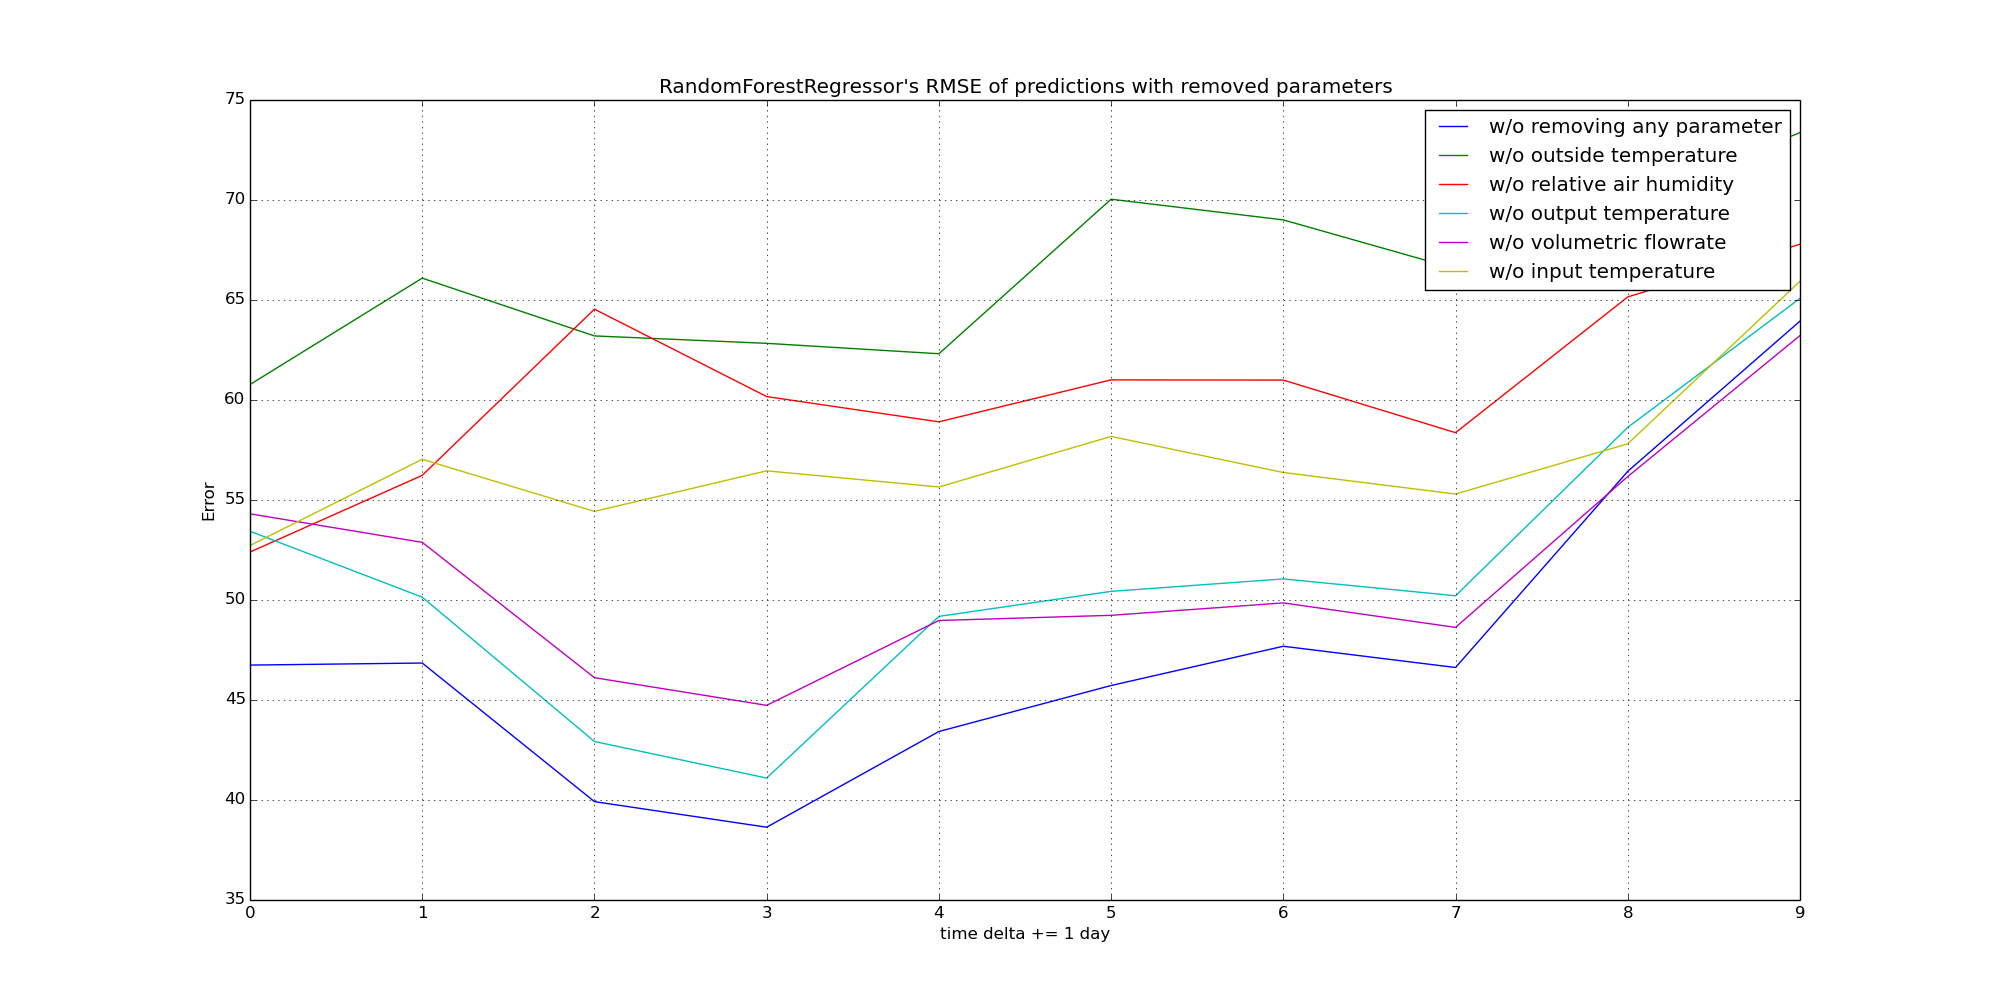
\includegraphics[width=1\linewidth]{img/RandomForestRegressor_day_error_without_some_params.png}
  \caption{Random Forest with effect of removing each parameter}
  \label{fig:RandomForestRegressor_day_error_without_some_params}
\end{figure}

\begin{figure}[H]
  \center
  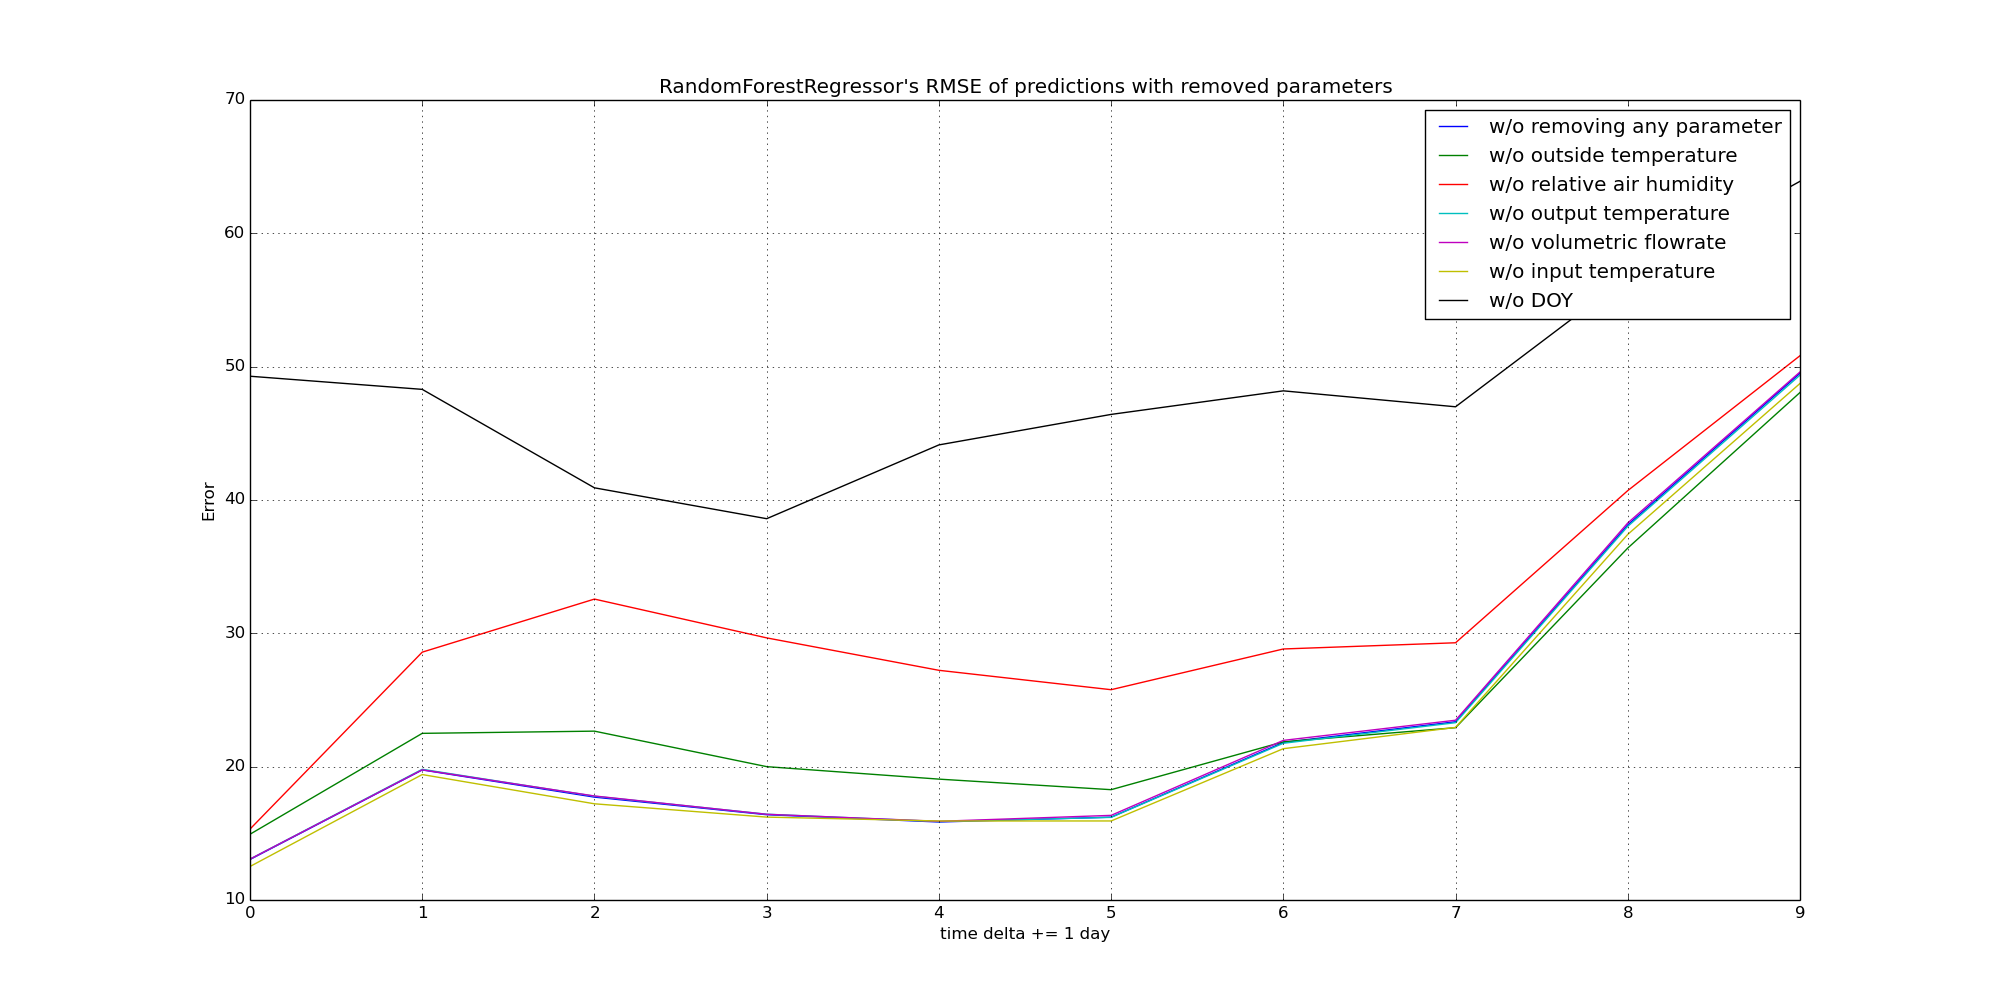
\includegraphics[width=1\linewidth]{img/RandomForestRegressor_day_error_without_some_params_DOY.png}
  \caption{Random Forest with Day of the Year information}
  \label{fig:RandomForestRegressor_day_error_without_some_params_DOY}
\end{figure}


\subsection{Exclusion of precipitation}	
%TODO
During analysis we assessed the importance of features, to study this we removed each feature and plotted the (Root Mean Squared Error)RMSE of the predictions it can be seen form the figure \ref{fig:RandomForestRegressor_day_error_without_precipation} that their is little or no effect on RMSE without precipitation.

\begin{figure}[H]
  \center
  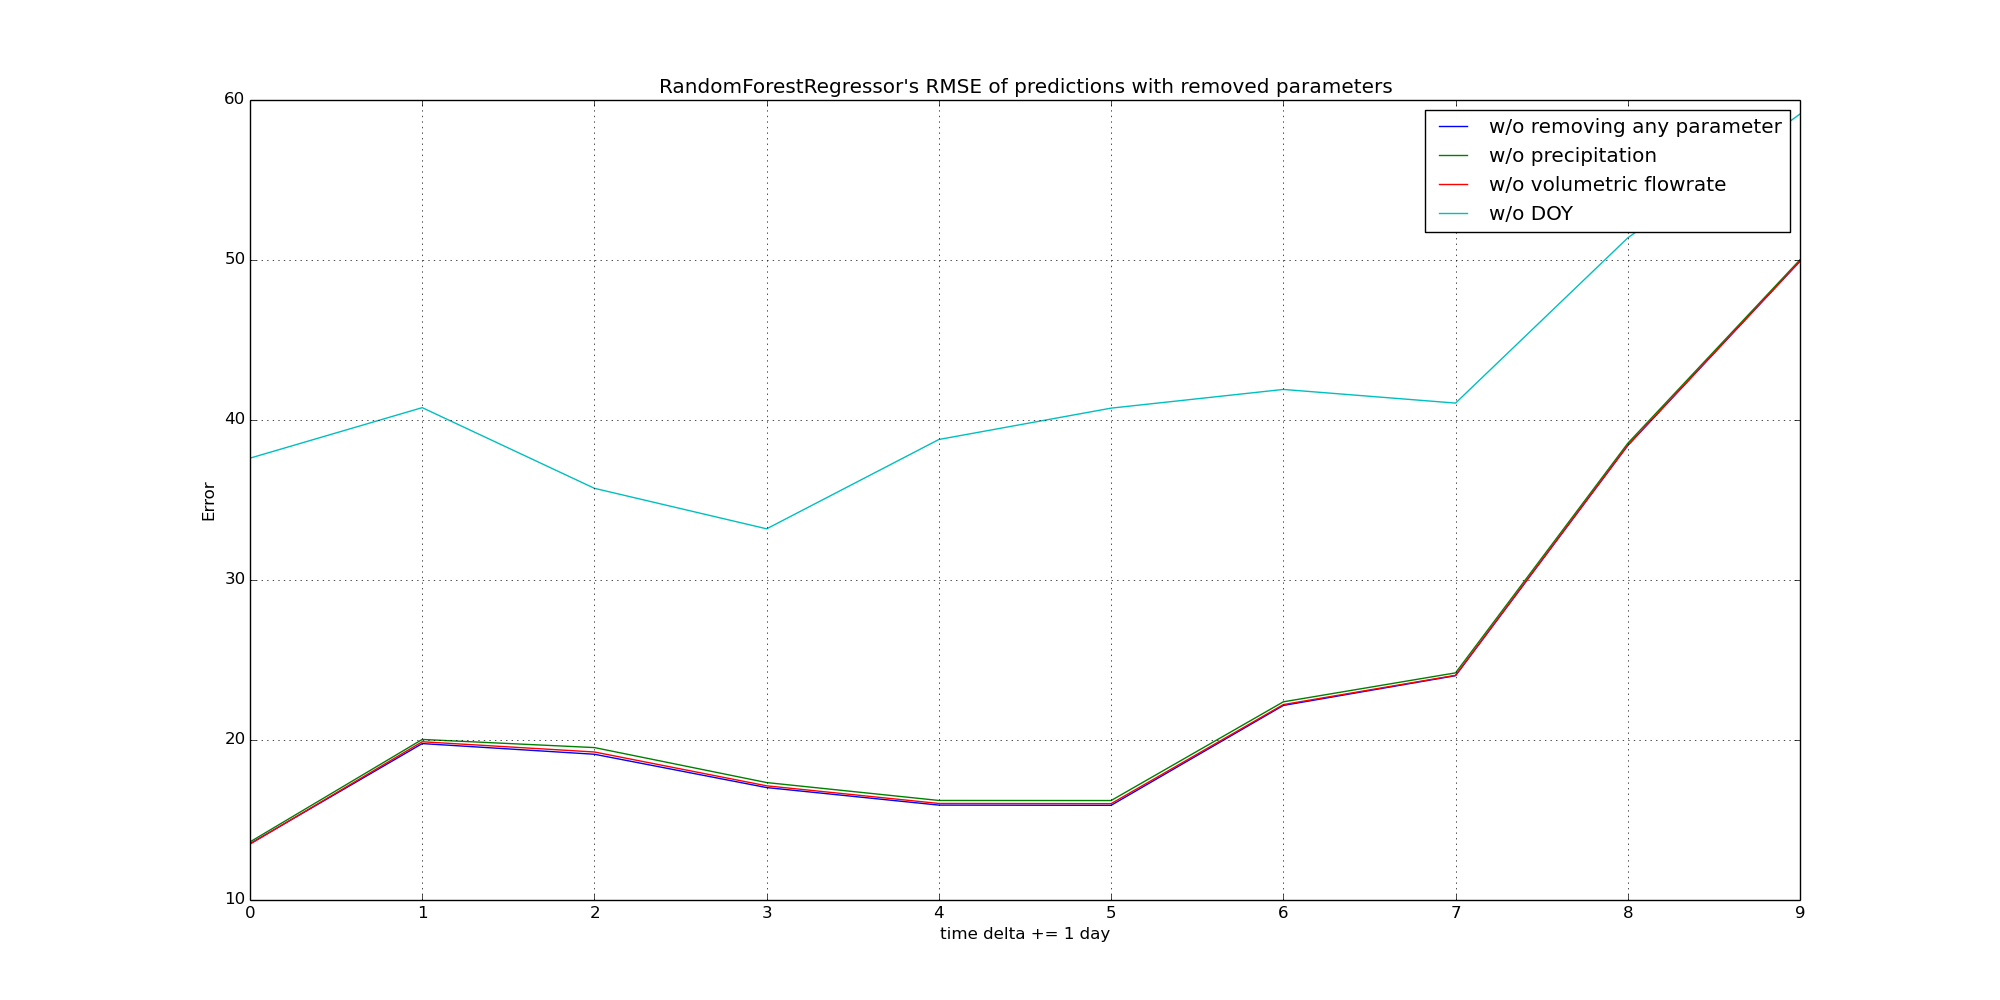
\includegraphics[width=1\linewidth]{img/RandomForestRegressor_day_error_without_precipation.png}
  \caption{Random Forest without Precipitation}
  \label{fig:RandomForestRegressor_day_error_without_precipation}
\end{figure}

\section{Methods}
\label{sec:methods}
To find an optimal prediction, we analysed two methods: For the gradient boosting we took a standard implementation and looked for optimal parameter, where for the time shifting window approach we focussed on the preprocessing of the data.
%TODO

\subsection{sliding window}
%TODO timeframe analysis

%TODO check read
As suggested in \cite{vafaeipour2014application} the sliding window approach was used to learn how to predict. In this approach the time series is split into windows or frames of input and output. Unlike in regression learning, those windows are shifted. Thus the learning algorithm does not learn the relation of the features at the same time, but their relation in the future. With this approach, it is possible to include all features as an input and select few of them as an output. This can be enhanced further by including predictable features into the input. These three methods are depicted in Figure \ref{fig:slidingwindow}.\\
The random forest implementation we are using however can not handle input with more than one dimension. Thus we flatten the input to one dimension. Since the feature values are typically easily separable, we expect the random forest to recognize this flattening in an early step. We do not include this as an extra information into the trees.
\begin{figure}[H]
  \center
  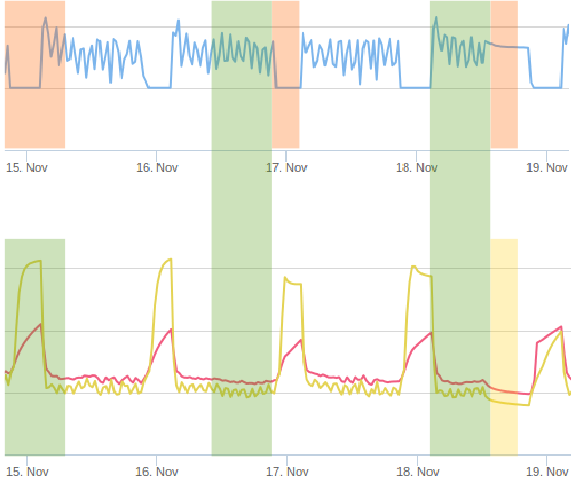
\includegraphics[width=0.6\linewidth]{img/regpred.png}
  \caption{Input(green) and output(red) frames for regression(left), prediction(middle) and enhanced prediction(right).}
  \label{fig:correlation}
\end{figure}

\subsection{gradient boost}
%TODO

\section{Conclusion}
\label{sec:conclusion}
%best result:
%sliding window with DOY
%Prediction output
\begin{figure}[H]
  \center
  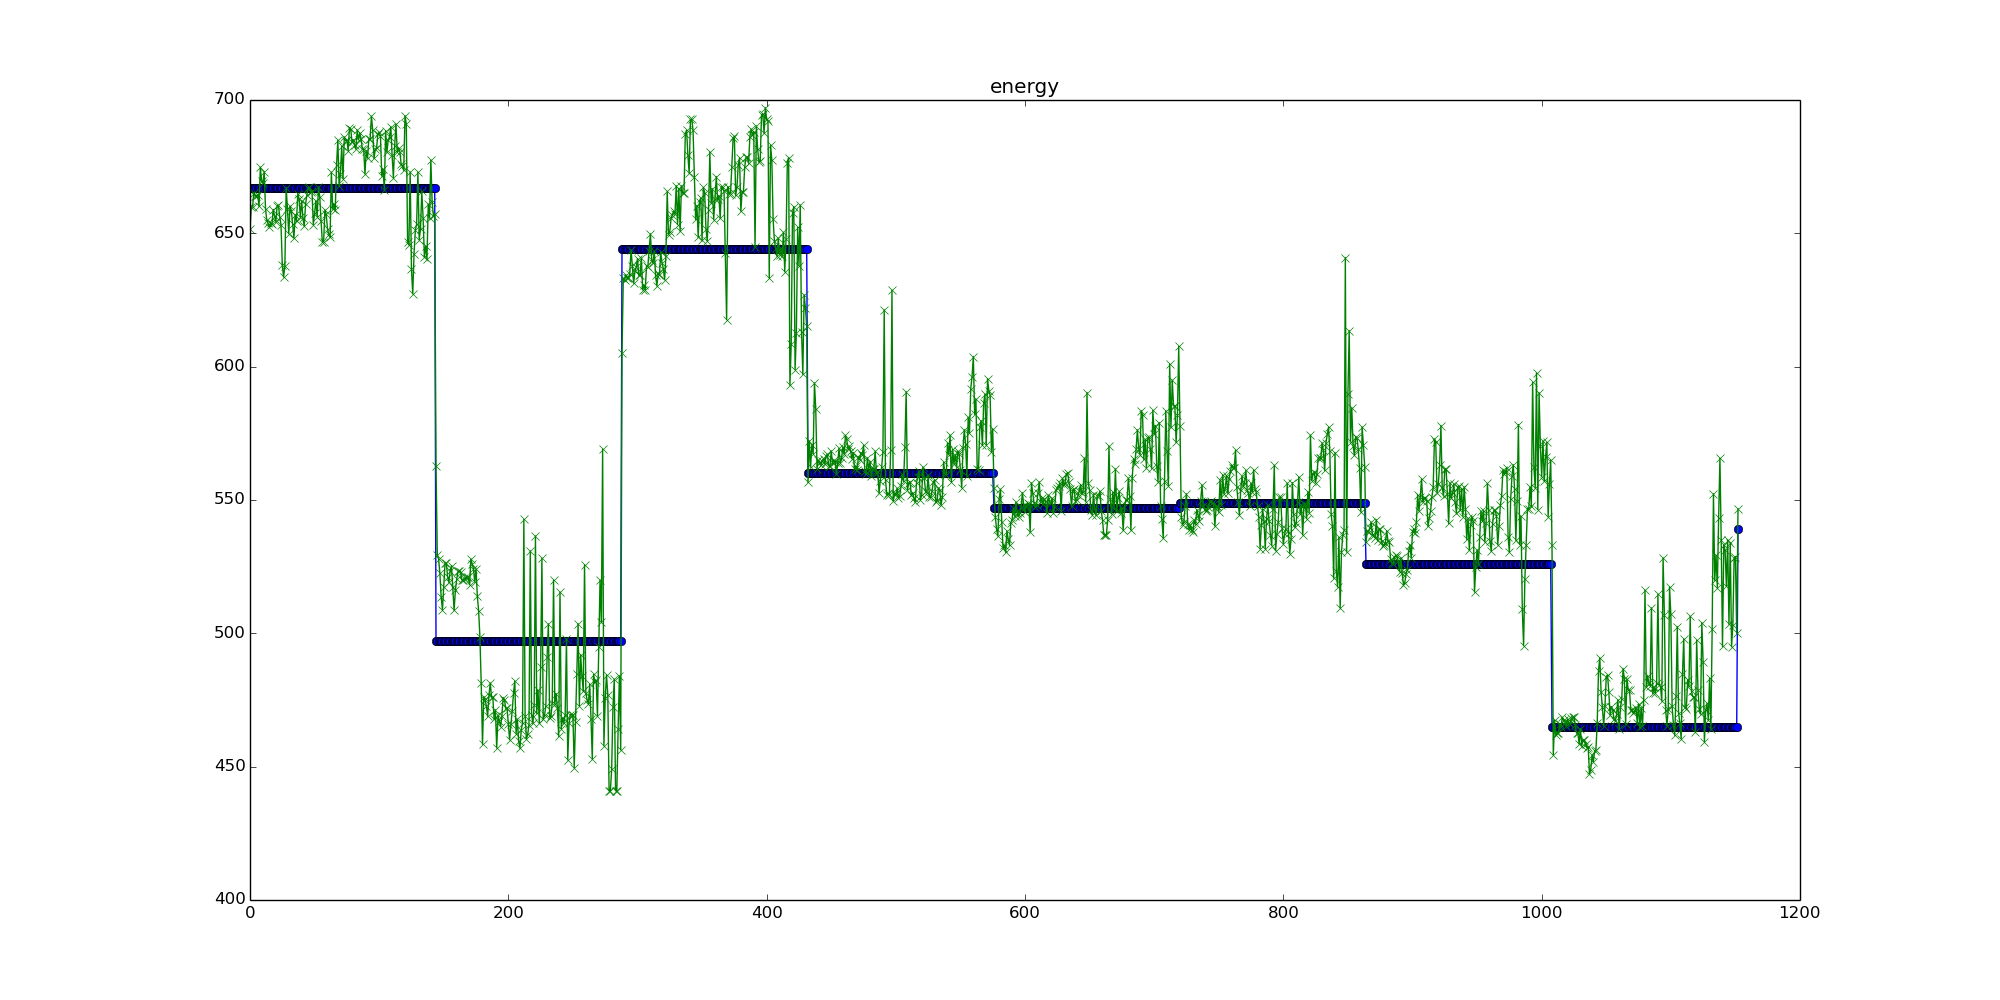
\includegraphics[width=0.6\linewidth]{img/predict-energy--0p890.png}
  \caption{Prediction of the energy using the sliding window approach.}
  \label{fig:Prediction}
\end{figure}

%score/error
%application conclusion


%BIBLIOGRPAHY
%TODO: check and fill the bibliography
\bibliographystyle{plain}%amsalpha
\bibliography{bib.bib}
%\bibentry{}

%\begin{appendix}
%\section{}

%\end{appendix}


%COPY AND PASTE FROM HERE

%\begin{enumerate}
% \item
%\end{enumerate}

%\href{link}{text}

%\begin[Language=Python]{lstlisting}
%#PYTHON CODE HERE
%\end{lstlisting}

%\lstinputlisting[language=Python]{	}

%\csvautotabular[separator=semicolon]{data.csv}


%\begin{figure}[H]
%  \centering
%  \includegraphics[width=0.5\linewidth]{../img/	}
%  %\caption{}
%  %\label{fig:}
%\end{figure}
%PUT UNITS ON THE FIGURES

\end{document}
